\chapter{Marco Teórico}
\label{marcoteorico}

El tema del emprendimiento no solo ha proporcionado ideas para la creación de películas cinematográficas o series de televisión. Como apoyo a los cursos formativos sobre emprendimiento han surgido multitud de juegos para enseñar y aplicar de forma práctica conceptos sobre la creación de iniciativas empresariales.

Estos juegos son una parte importante de la formación ya que permiten aprender de forma más amena. Además el utilizar de forma práctica los conocimientos adquiridos ayuda a que se entiendan mejor y se recuerden durante más tiempo.

Para los juegos mencionados anteriormente existen varios formatos que serán explicados en detalle a continuación. 

\section{Actividades en grupo}

Es el tipo más sencillo y tradicional. Solo necesita de los participantes y una actividad previamente elegida. Una de las ventajas que tiene este tipo de actividades es que ponen a las personas en contacto directo, de modo que tienen que dejar a un lado la vergüenza e interactuar como lo harían ante clientes, inversores o trabajadores. Además estos encuentros pueden servir para hacer contactos útiles en un futuro.

Este tipo de actividades potencian las habilidades sociales y la creatividad de los participantes ya que los únicos elementos del juego son las personas, y las mecánicas del juego son sus discursos, explicaciones, gestos, actuaciones, etc.

\section{Juegos de mesa}

Los juegos de mesa mantienen muchos de los aspectos positivos de las actividades en grupo ya que también son presenciales, con las ventajas y desventajas que ello conlleva.

Además estos juegos pueden ser más divertidos debido a que introducen elementos como tableros, cartas, textos o ilustraciones entre otros elementos. Son especialmente interesantes para personas que no se sientan cómodas con las actividades en grupo debido al alto grado de interacción que demandan.

También es más fácil el uso de mecánicas complejas ya que hay instrumentos para contabilizar y describir el estado del juego: dados para contar el número de vidas, poder mágico o turnos; tableros con diferentes casillas, territorios o zonas; fichas de jugador con parámetros, habilidades, y características.

Actualmente hay numerosos juegos de mesa entre los que destacaremos:
\begin{description}
\item[Colonos de Catán: ] (figura \ref{catan})  Apto para 6 jugadores (a través de una expansión), este juego de gestión de recursos y comercio nos pone en la piel de un colono que debe ir construyendo sus aldeas y caminos. En Colonos de Catán prima tu habilidad para negociar por el contrario y tu capacidad de estrategia a medio y largo plazo. \cite{faceentrepreneurship2016}

El Catán [...] evita el enfrentamiento tan directo y obliga a negociar para ganar.

Ahí reside una de las claves, en el hecho que de entrada nadie posea recursos suficientes de todos los tipos para progresar. En cada turno se comercia con las materias primas, un trueque básico que permite saber cómo funciona un mercado libre en el que cada uno tiene sus propios intereses. \cite{albertini2015}

Lleva unas 18 millones de copias vendidas [...] Ha aparecido en \textquote{The Big Bang Theory} [...] Mark Zuckerberg se ha declarado adicto, \textquote{es uno de esos juegos a los que debes jugar si no quieres ser el \textquote{margi} de Silicon Valley} \cite{albertini2015}

\begin{figure}
\begin{center}
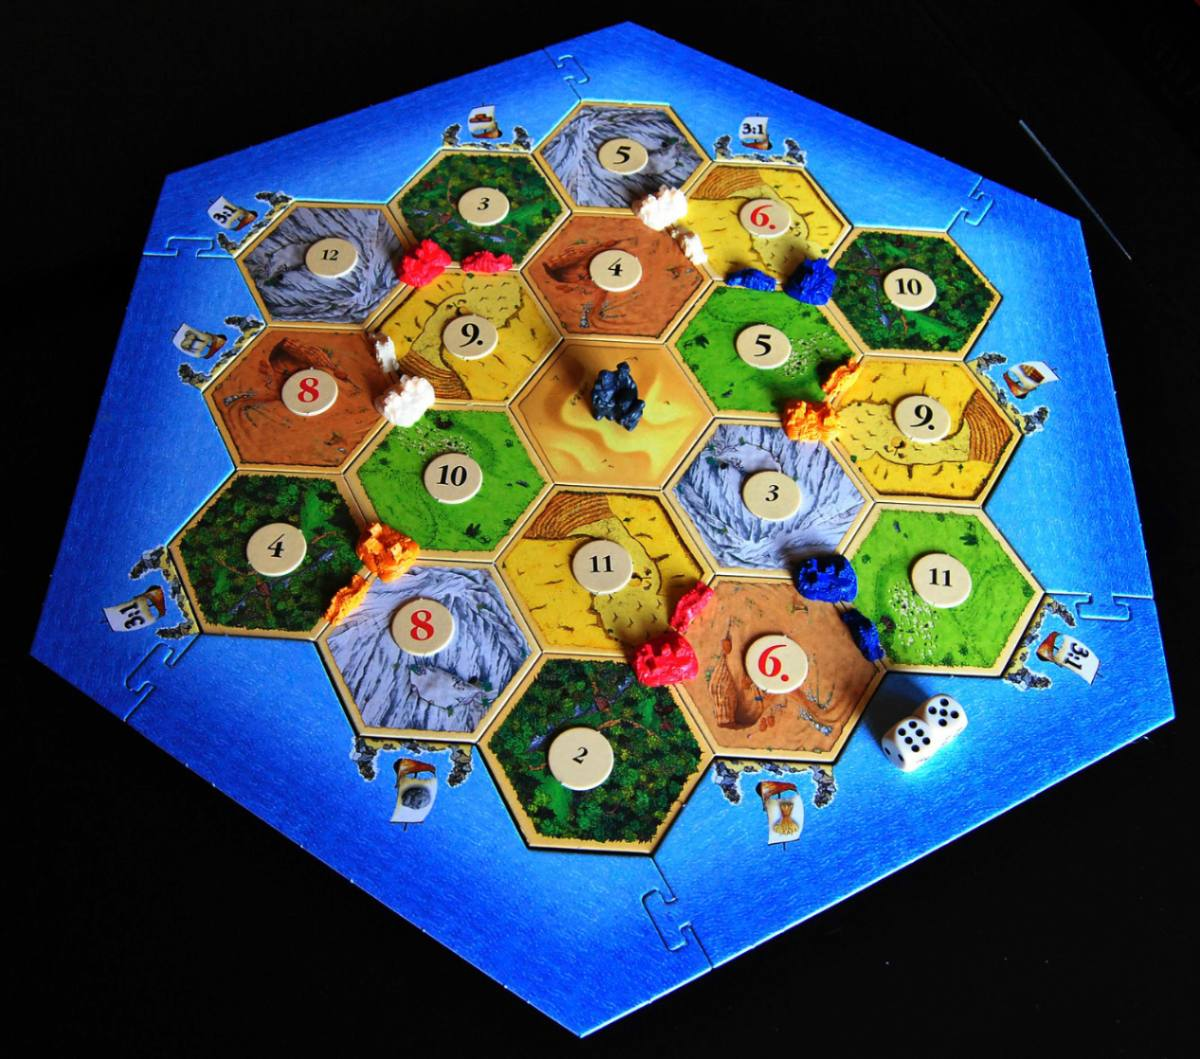
\includegraphics[scale=0.3]{imagenes/catan.jpg}
\caption{Tablero del juego Colonos de Catán}
\label{catan}
\end{center}
\end{figure}


\item[Pandemia: ] (figura \ref{pandemia}) En Pandemia somos un grupo de hasta 4 científicos que tienen que mantener a raya una serie de virus, o de lo contrario la Humanidad tendrá un grave problema. [...] debes aprender a formar equipo y hacerlo funcionar si quieres tener éxito en tu \textquote{startup}. En este sentido, Pandemia puede ser la terapia perfecta para ti y tu equipo ya que o colaboráis y funcionáis perfectamente engrasados o correréis el riesgo de fracasar. Y también en la vida real. \cite{faceentrepreneurship2016}

\begin{figure}
\begin{center}
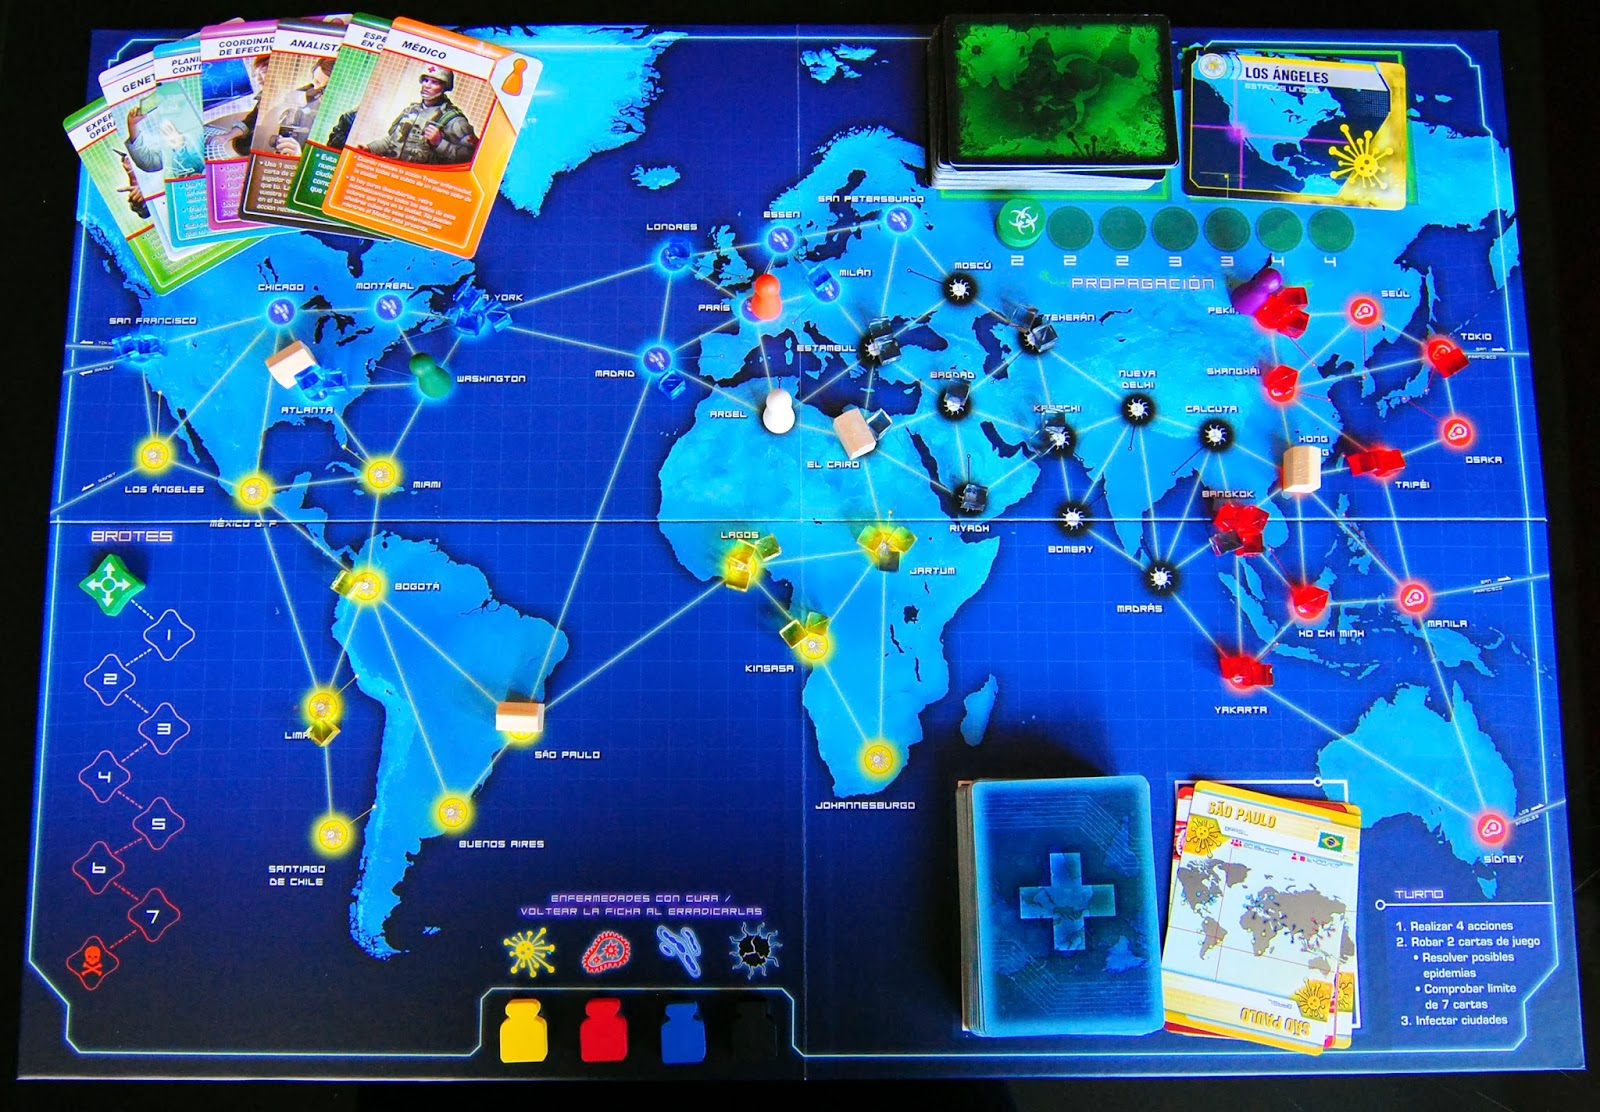
\includegraphics[scale=0.25]{imagenes/pandemia.jpg}
\caption{Tablero del juego Pandemia}
\label{pandemia}
\end{center}
\end{figure}

\item[Flea market:] (figura \ref{fleaMarket}) Juego de dados en el que tendrás que descubrir los tesoros escondidos en un mercado de segunda mano. Tú serás el cliente que compra, y tu objetivo es adquirir bienes lo más barato posible para venderlos por más dinero una vez el dado de la demanda dice que ya son populares de nuevo. \cite{mariagonzalez2015}

\begin{figure}
\begin{center}
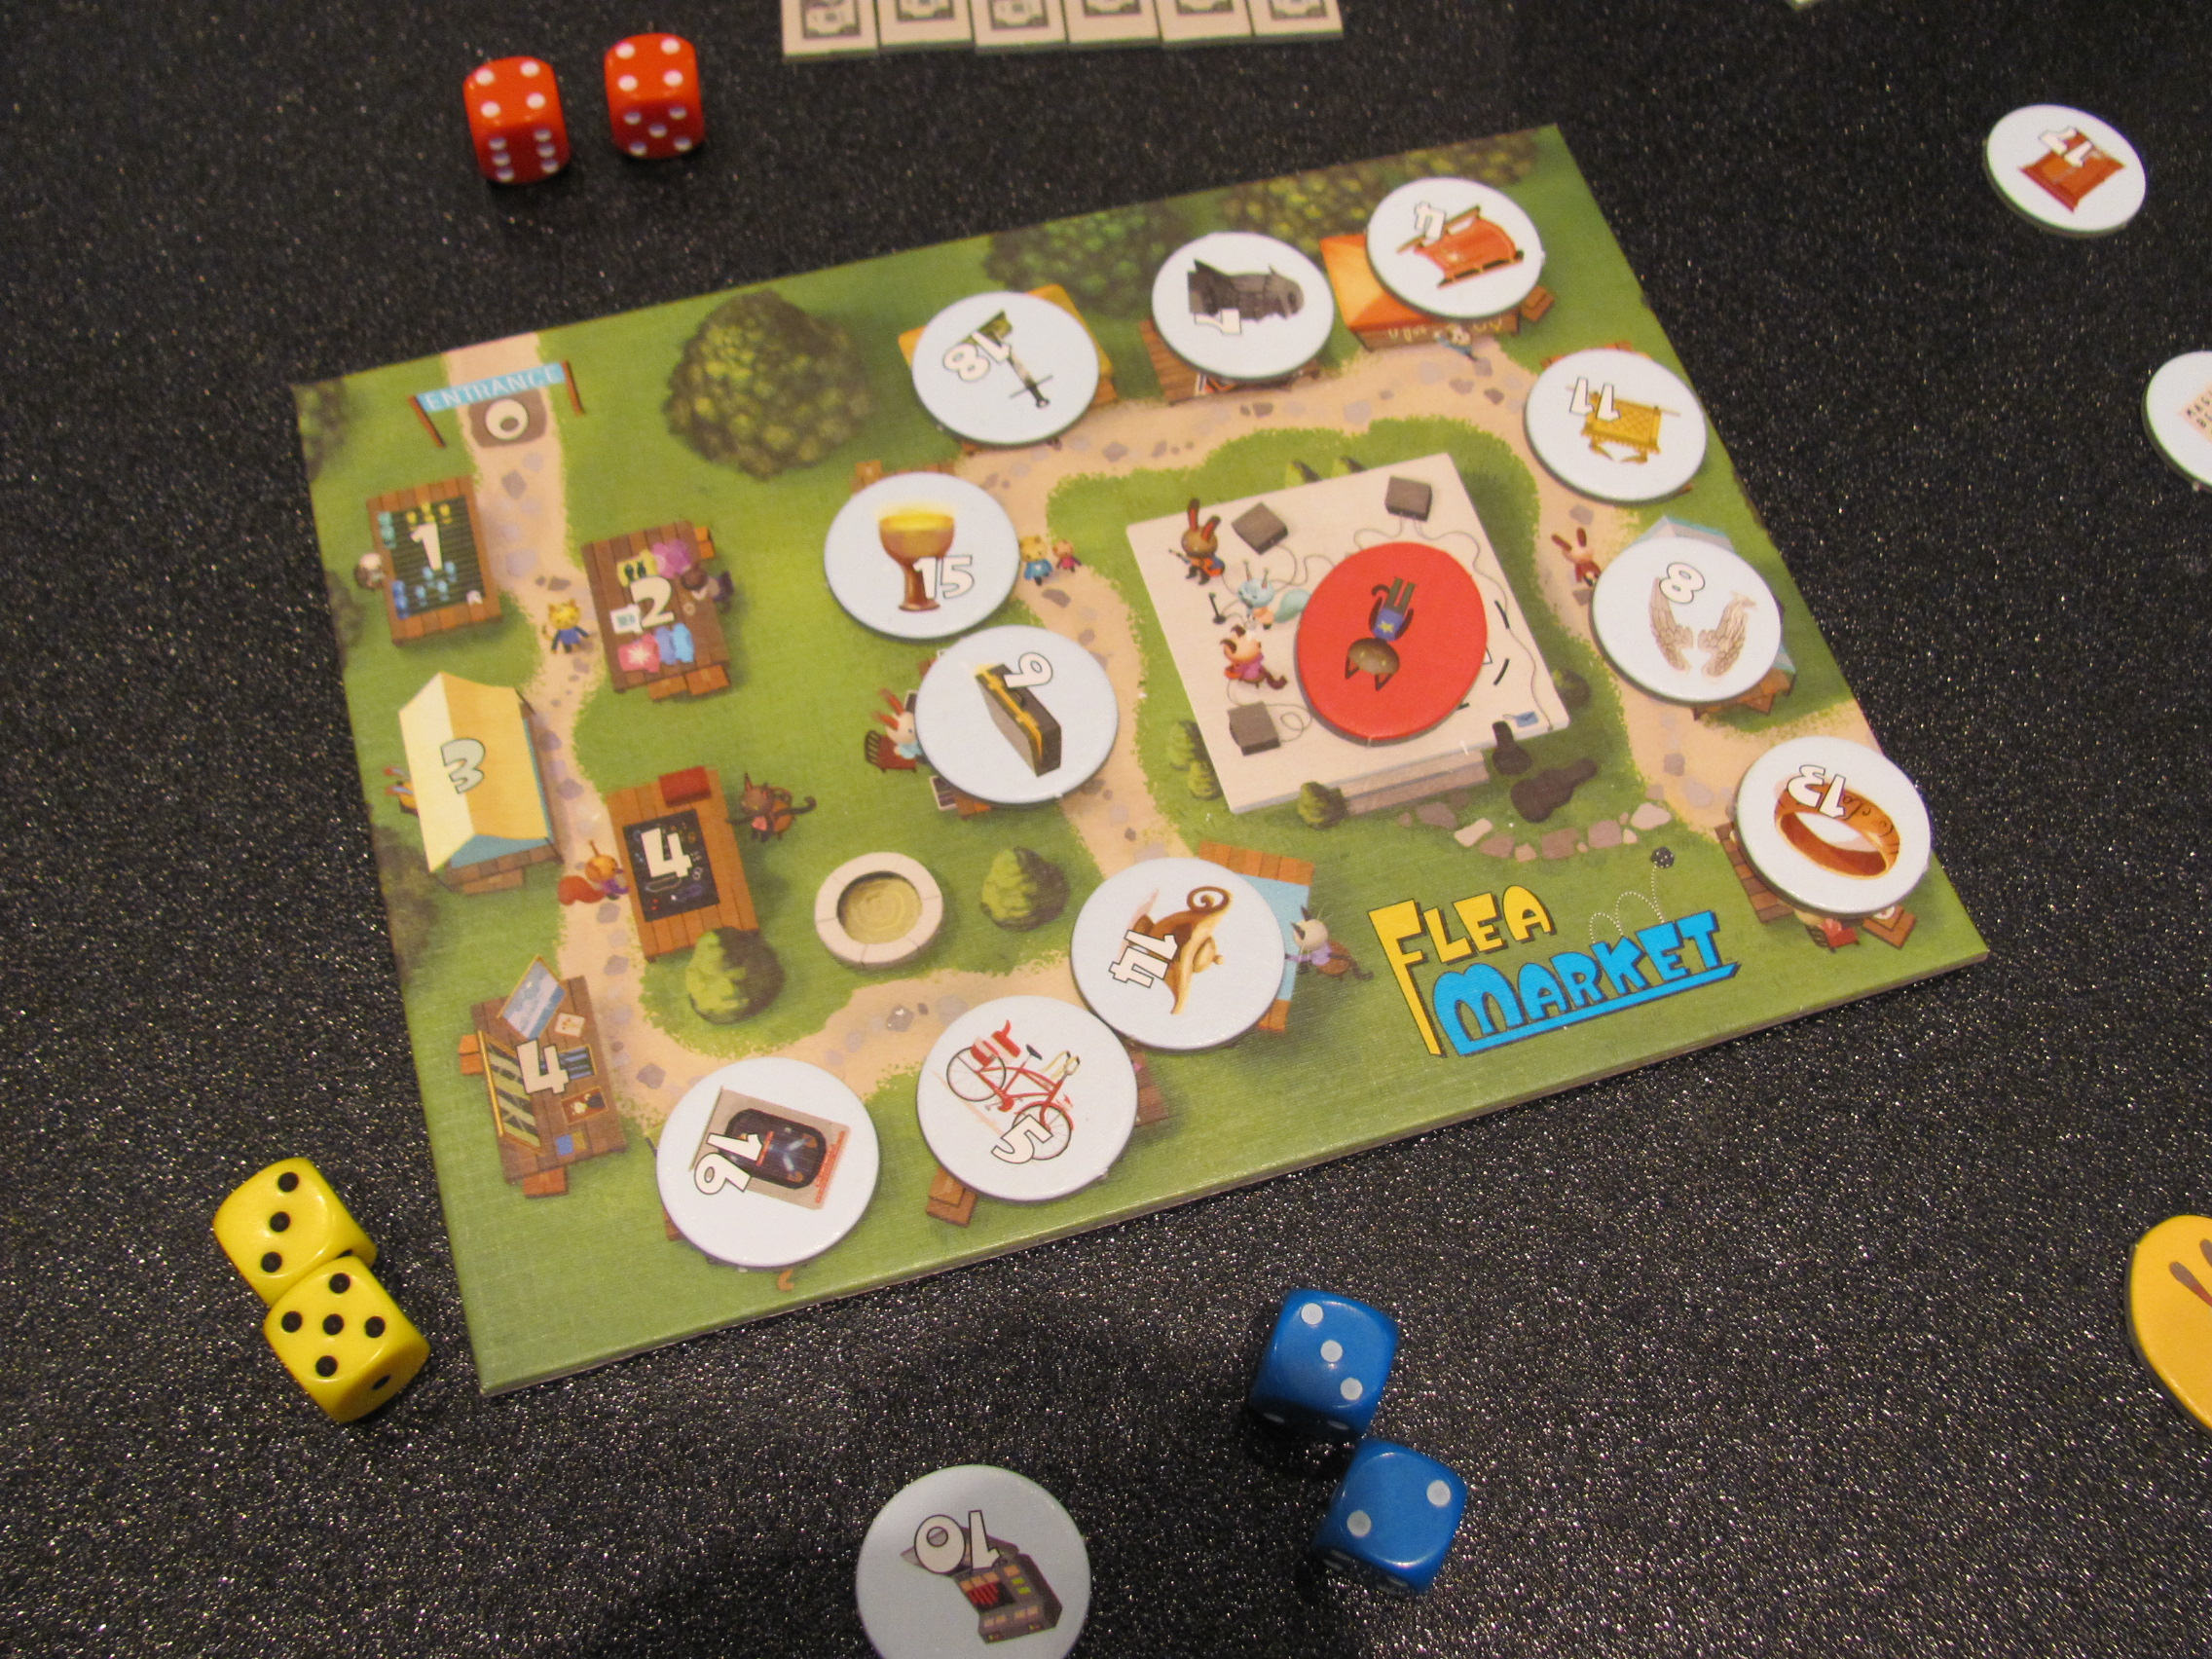
\includegraphics[scale=0.4]{imagenes/fleaMarket.jpg}
\caption{Tablero del juego Flea market}
\label{fleaMarket}
\end{center}
\end{figure}

\end{description}


\section{Videojuegos}

Con el creciente éxito del mercado de los videojuegos y el entretenimiento digital, los videojuegos sobre el emprendimiento no se han hecho esperar. Los hay de diferentes tipos y temáticas aunque todos ellos comparten la esencia de dirigir un negocio.

\begin{description}
         \item[Gestionar un negocio:] en este tipo de videojuegos el jugador es el gerente de un negocio como por ejemplo una cafetería o una peluquería. El objetivo es gestionar la actividad diaria del establecimiento y ampliar el mismo utilizando los ingresos obtenidos. Ejemplos de este tipo de videojuegos son \textquote{Diner dash} o \textquote{My Cafe: Recipes \& Stories}. Este tipo de juegos tienen un carácter más infantil y recreativo y distan de ser un juego basado realmente en el emprendimiento y el mundo \textquote{startup}. El motivo es que el peso del juego reside principalmente en la gestión cotidiana del negocio como servir pedidos, cobrar a los clientes o comprar materiales; valores muy importantes para el emprendedor como la creatividad, la estrategia, la pasión o la innovación no suelen tener cabida en estos juegos.
         
%pon alguna URL de estos videojuegos al pié de la página 

	\item[Hipster CEO:] (figura  \ref{hipster01}) este juego se puede considerar la contraposición al juego mencionado en el punto anterior ya que elimina las tareas de interacción directa con el cliente y en su lugar el jugador se centra en la gestión desde un punto de vista más técnico. El objetivo de este juego es lanzar y dirigir una \textquote{startup} con todo lo que ello conlleva.
	
Entre las tareas del jugador se pueden destacar: contratar personal, dedicar recursos a los diferentes departamentos (ventas, producción o marketing) 

Para ello se dispone de un dashboard con varias \textbf{métricas clave} sobre la \textquote{startup} que ayudan al jugador a tomar decisiones acerca del rumbo de la misma. El juego no dispone de ningún tipo de historia o personajes que controlar, si no que la interacción con el mismo es a través de informes, dashboards, emails, etc.

\begin{figure}
\begin{center}
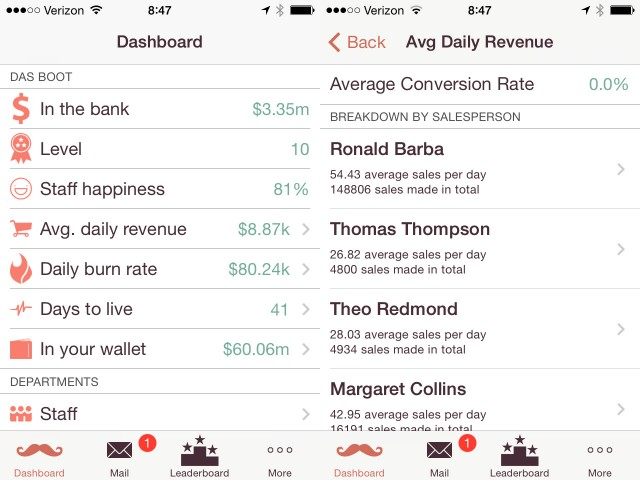
\includegraphics[scale=0.6]{imagenes/hipster01.jpg}
\caption{Captura de pantalla de iPhone con el juego Hipster CEO}
\label{hipster01}
\end{center}
\end{figure}

	\item [U-startup:] (figura \ref{ustartup01}) es un juego desarrollado por la Universidad de Cádiz en España, en colaboración con la Cátedra de Emprendedores y OmniumLab. Lo novedoso de esto es que es el primer videojuego sobre emprendimiento con el que aprenderás a construir tu negocio con la metodología de CANVAS. \cite{danieladelbosque2016}
	
Este juego se puede considerar la contraposición a los juegos mencionados en el punto anterior ya que explícitamente se muestran elementos típicos de la metodología \textbf{lean startup} tales como el \textbf{lean canvas}. El juego se basa en completar este canvas con las hipótesis de negocio del jugador a la vez que se completa una aventura en la que un fantasma es el mentor del jugador en el mundo empresarial, la pitonisa ayuda a encontrar los clientes objetivo y otros personajes y escenarios intervienen.
	
\begin{figure}
\begin{center}
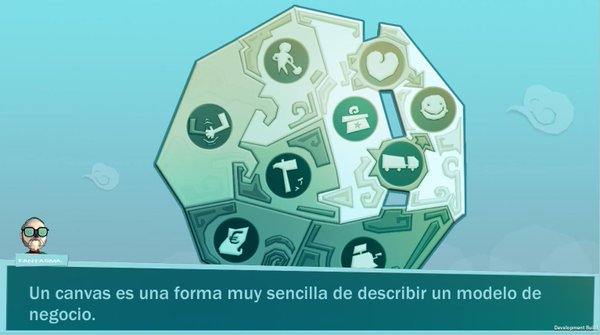
\includegraphics[scale=0.6]{imagenes/ustartup01.jpg}
\caption{Vista del lean canvas en el juego U-startup}
\label{ustartup01}
\end{center}
\end{figure}

\end{description}